\documentclass{article}
\usepackage[utf8]{inputenc}
\usepackage{float}
\usepackage{graphicx}
\usepackage{gensymb}

\title{Rover Advancements - Ceres}
\author{Nicolas Correal Murillo \and Juan Felipe Ruiz Sosa}
\date{\today}

\begin{document}

\maketitle

\section*{Introduction}
We, the Ceres team, are developing a Martian exploration rover to participate in international competitions.
Our project aims to expand our knowledge in various technical fields and demonstrate the expertise we've gained
 through past robotic experiences and our professional careers. By tackling the challenges of designing and 
 building a rover capable of operating on Mars, we hope to advance our skills and contribute to the broader 
 field of space exploration. We differentiate our selves with this proyect by being the only team developing our own motors from scratch.


In this document we highlight our most relevant milestones, along with the main developments and learnings along the way, as well stating with our following steps.

\tableofcontents

\section{Milestones Achieved}
 \subsection{Motors}

 \subsubsection{First prototype}
\paragraph{Developments}
 \begin{itemize}
    \item 100mm x 10mm Stator - 3 phase Winding
    \begin{figure}[H]
        \centering
        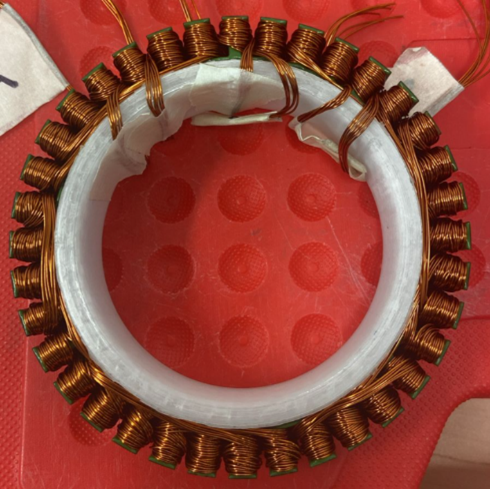
\includegraphics[scale=1.5]{Images/Estator10010PrimerEmbobinado.png}
        \caption{First Motor Winding}
    \end{figure}
    \item 3D model of the rotor with 42 poles (magnets) along with a base
    \item 3D Print of the motor and assembly
    \item Initial test with a 30A generic ESC
 \end{itemize}
\paragraph{Results}
\begin{itemize}
    \item The motor vibrates, like triying to move
    \item The motor winding heats up a lot and very quickly as soon at it is turned on
    \item The rotor sticks to one side of the stator as it is not supported by anything at its center
    \item 2 ESC were broken due to the high current draw
\end{itemize}
\paragraph{Conclusions}
\begin{itemize}
    \item The motor base needs to have an alligment that mantains the rotor at the center of the structure
    \item An ESC with higher current capacity is needed for these tests.
    \item It is necessary to check why one of the phases was heating up to 105\degree C. As well as identifying if this was the cause of the motor not being able to spin
\end{itemize}


\subsubsection{Second prototype}
\paragraph[short]{Development}
\begin{itemize}
    \item A new motor was designed, featuring a rotor (upper part) with an extension that fit into an internal base within the stator (lower part), 
    which blocked lateral movement and limited vertical position while allowing rotational movement. Both parts were made entirely of plastic.
    \item The motor winding was redone because we found that some of them were wound in the opposite direction to what they should have been. 
    This caused the magnetic field, responsible for generating rotation, to be constantly canceled out.
    \item 3D printing and assembly
\end{itemize}

\paragraph{Results}
\begin{itemize}
    \item An 80A 6S ESC was used in order to use higher voltage and current when trying the motor. 
    \item The motor spins correctly, however no cuantitative methods were used to classify the success of this movement.
    \item After some time of testing, the friction between the internal support of the rotor and base of the stator make them melt together.
    \item The rotor still isnt maintained correctly in the vertical axis.
\end{itemize}
\paragraph{Conclusions}
\begin{itemize}
    \item A different alternative to maintain the rotor aligned is neccessary. One that reduces friction while maintaining the center firmly in its position.
\end{itemize}

\subsubsection{Third Protoype}


\paragraph[short]{Development}
\begin{itemize}
    \item A new 3D design of the base was created, where the connection between the base and the rotor is made using a bearing to reduce friction and improve the rigidity of the coupling between the two parts.
    \item An arm was designed for the rotor, which will help us have a basic understanding of the torque the motor can produce.
    \item The rotor design was changed so that the magnets are no longer attached with resin, allowing for faster and more efficient assembly and facilitating the effective recovery of the magnets for use in future prototypes.
    \item Printing and Assembly of the model
    \item Speed was measured with a tacometer
    \item Current was measured with a current clamp at no motor load
    \item Simple cualitative torque tests
\end{itemize}

\paragraph[short]{Conclusions}
\begin{itemize}
    \item The speed measured with the tacometer doesnt seem to be accurate, as it gave a far faster speed than expected (4000rpm vs 2000rpm) and after that failed to read in further tests.
    \item The motor visibly has an easier time spinnign with the bearing, as friction was greatl reduced
    \item Another way to measure the motor speed is neccessary.
    \item We need a cualitative and more safe way to measure the torque output.
\end{itemize}

\subsubsection{First Cycloidal Drive prototype}
\paragraph[short]{Development}
\begin{itemize}
    \item A cycloidal drive was designed to fit within the stator of the motor, thereby optimizing its volume. This gearbox features a central shaft (highlighted in the photo) which is anchored to the motor rotor. As it rotates, the discs on the shaft (highlighted in the photo) turn with the desired reduction ratio due to the shape of the ring (highlighted in the photo). To capture this reduction, the discs have holes through which the output shaft (highlighted in the photo) is inserted, rotating with the expected reduction ratio, which in this case is 8:1. Thus, for every 8 turns of the rotor, the output makes 1 turn, but with greater torque.
    \item Some parts were printed to test the concept with bearings and screws, and to adjust the design based on the results.
    \item The entire prototype was 3D printed in plastic and assembled with bearings and screws.
    \item Tests were made to verify that the expected reduction in terms of rotations was being achieved.
\end{itemize}
\paragraph[short]{Results}
\begin{itemize}
    \item The cycloidal drive was operational.
    \item The expected reduction ratio of 8:1 in terms of rotations was achieved.
    \item Some screws collided due to the dimensions of the parts and the screws themselves, causing friction that hindered the gearbox's movement.
    \item The alignment method was insufficient, causing the gearbox to twist during operation.
\end{itemize}

\paragraph[short]{Conclusions}
\begin{itemize}
    \item Details such as the sizes of the parts and screws need to be adjusted so that tolerance does not interfere with the movement.
    \item The efficiency of torque transmission in the reduction needs to be calculated.
    \item With the necessary adjustments, the cycloidal drive will be ready to be assembled with the motor for testing maximum torque, speed, and consumption.
\end{itemize}

\subsubsection{First \textbf{Internal} Cycloidal Drive prototype}
\paragraph[short]{Development}
\begin{itemize}
    \item A design was created to connect the rotor (motor output) to the cycloidal drive shaft (gearbox input) located within the stator to optimize motor volume. Additionally, an external base was designed to cover the motor and support and stabilize the cycloidal drive output.
    \item The entire prototype was 3D printed in plastic and assembled with bearings and screws.
    \item Tests of motor and the cycloidal drive movement were made with this new design.
\end{itemize}
\paragraph[short]{Results}
\begin{itemize}
    \item The Internal Cycloidal Drive was operational.
    \item Some parts were too close together, causing friction and slightly hindering the motor's movement.
    \item The base lacked a component to prevent unwanted rotation of the cycloidal drive shaft, causing the motor to stop on some occasions.
\end{itemize}

\paragraph[short]{Conclusions}
\begin{itemize}
    \item Tolerances and the placement of some screws need to be corrected in the design to prevent collisions.
    \item A component should be implemented to keep the cycloidal drive shaft stable.
    \item Since the motor operates with its cycloidal drive, it is necessary to conduct speed and torque tests on the next prototype. Therefore, a test setup with the necessary sensors should be designed to obtain these data.
\end{itemize}

\subsubsection{Second \textbf{Internal} Cycloidal Drive prototype}
\paragraph[short]{Development}
\begin{itemize}
    \item A new prototype of the Internal Cycloidal Drive was designed, in which the screws on the output shaft holding the bearings were replaced with steel pins to support bushings, improving its stability. Additionally, sizes and distances between parts were corrected to prevent friction and reduce motor performance. A cover was also implemented on the base to stabilize the rotor and the cycloidal drive shaft.
    \item The entire prototype was 3D printed in plastic and assembled with bearings, bushings. steel pins and screws.
    \item 
\end{itemize}
\paragraph[short]{Results}
\begin{itemize}
    \item
\end{itemize}

\paragraph[short]{Conclusions}
\begin{itemize}
    \item
\end{itemize}

\section{Future Goals and Objectives}
Outline upcoming milestones and targets for the project, discussing the expected impacts and contributions to the broader field of space exploration.

\section{Investment Opportunities}
Detail how investors can contribute to the project, emphasizing potential returns and strategic benefits for stakeholders.

\section*{Conclusion}
Summarize the project's importance and reiterate the call to action for potential investors, encouraging their participation and support.

\end{document}
